\documentclass[a4paper,10pt,twocolumn,uplatex]{jsarticle}
\usepackage{style/nislab,style/resume}

%---------------------------------------------------------------------
% レジュメ種別・日付設定(要変更)
% \type{} 1:修士論文諮問会 2:卒業論文発表会 else:月例発表会
\type{5}
\year{2021}
\month{11}
\date{16}

%---------------------------------------------------------------------
% ページ番号設定(要変更)
\setcounter{page}{1}

%---------------------------------------------------------------------
\begin{document}
%---------------------------------------------------------------------
% タイトル作成部分(要変更)
% \maketitle{タイトル}{title}{名前}{name}
\maketitle{ARによるドローンの動作意図の伝達}
{Communicating Robot Motion Intent with Augmented Reality}
{竹内 一真}
{Kazuma Takeuchi}
{杉本 涼輔}
{Ryosuke Sugimoto}


%---------------------------------------------------------------------


\section{はじめに}
効果的なコラボレーションのためには,チームメイトが自分の意図を迅速かつ正確に伝え,共通の基盤を築く必要がある.
中でも,社会科学,認知科学,行動科学の先行研究によると,協調的な活動は基本的に相互予測可能性
% (各チームメンバーがチームメイトの態度や行動を迅速に理解し,予測する能力)
に依存していることがわかっている.特に人間とロボットが混在するチームでは,ロボットの意図の伝達がうまくいかない場合,安全性,タスクパフォーマンス
等を低下させる故障につながる可能性がある.
そのため,チームメイトのロボットがいつ,どこで,どのように動くのかをユーザが理解しやすくすることは
安全で使いやすいドローンシステム実現のための課題である.
% 人間同士のチームでは,視線やジェスチャー,その他の社会的行動など,さまざまな暗黙的・明示的な手掛かりを用いて,
% 計画された行動や動作を伝え,チームの効果を高め,信頼関係を維持しています.
% ドローンも社会的な手掛かりを用いて動作の意図や感情の状態を伝える可能性があることが研究で示されているが,
% これらの知見を産業用ドローンや空中ドローンなど
% 擬人化やズームアップの機能を持たないドローン
% に適用する方法は明確化されていない.
% その代替として
そこで近年のHRIの研究では,ロボットの動きの推論を支援する手法が模索されている.
% 読みやすい動きの軌跡の生成,表現力のあるモーションプリミティブの開発,自然言語を用いたドローンの意図の言語化,
% プロジェクタを用いた電子ディスプレイシステムによる追加情報の提供,
% 明示的な方向性の手がかりとしての光信号の使用などがある.

本論文\cite{main}ではAR(Augmented Reality)を利用し,特に空中ドローンにおいて,ドローンの動きの意図を同じ場所にいるユーザーに伝え,
動きの推論を行う手法を模索する.
% 本研究は,ARHMD(Augmented Reality Head-Mounted Displays)が,
% 同じ場所にいるユーザのための直感的な人間とドローンのコミュニケーションをサポートすることを想定している.
% 本研究では,このデザインスペースを,特に空中ドローンにおいて,ドローンの動きの意図を同じ場所にいるユーザーに伝えるという観点から,
% 初めて詳細に検討しました.

%---------------------------------------------------------------------


\section{提案手法}\label{discussion}
\subsection{概要}
% ARHMD技術が,ドローンの動作意図を提供することで,
% 人間とドローンのインタラクションをどのように強化するかを検討するためのデザインフレームワークを構築した.
ARHMDがどのように人とドローンのインタラクションを強化するかを検討するためのARインタフェースを構築した.
以下では,構築した4つのARインタフェースの特徴について述べる.
具体的なデザインは\figref{fig:arinterface}に示す.

\subsection{NavPoints}
NavPointsデザインではドローンの計画された飛行経路を,
いくつかの線と球体で表示する仮想イメージを提供する.
この仮想イメージではドローンの目的地であるウェイポイントを球体で表示し,
ドローンの現在位置とそれらの目的地を順に線で結ぶ.
% 3次元空間におけるドローンの正確な目的地であるウェイポイントは球体で表示さている.
% 3次元空間におけるドローンの正確な目的地を示す.
また,直下の地面には球体の影が描画され,ここからユーザは奥行きの推定を行う.
加えて,各球体の上には2つの放射状のタイマーが配置されており,
内側の白いタイマーはドローンがその場所に到着する時刻を,
外側の紺色のタイマーはドローンがその場所を離れる時刻を示す.
% 小さな球体が線に沿って移動し,ドローンが目的地の間を移動するのと同じ方向と速度で動くことで,
% 将来のドローンの速度と方向を予測する手がかりとなる.
このデザインは,速度や発着のタイミングに関する情報がユーザーに対して明示的に表示される.


%---------------------------------------------------------------------


\subsection{Arrow}
Arrowデザインの仮想イメージは青い矢印で構成されており,ドローンが数秒後に通ると推測される経路を示す.
% 矢印の頭の動きに合わせて,ドローンまでの矢印の軌跡を示す線が残されています.
% この線を利用して,
また,この矢印の直下には影が描画され,ユーザはこれらからドローンの経路を把握することが可能である.
% 先述のNavPointsデザインは多くの情報を提供する一方で,過剰な描画によりユーザの混乱を招く可能性がある.
本デザインはNavPointsよりミニマルなアプローチで,速度や発着のタイミングをユーザが推測する必要があるものの,
時間的な情報を伝えることに特化している.
% 表示される速度や到着/出発のタイミングなどの情報は,ユーザーが空間を通過する矢印の離散的な動きを見て推測する必要があります.
% NavPointsデザインはユーザーに多くの情報を提供する一方,過剰な描によりユーザの混乱を招く可能性がある.
% Arrowデザインは,よりミニマルなアプローチをとり,[8]や最新のGPSシステムでの一般的なユーザーの経験にヒントを得て,時間的な情報を伝えることに特化しています.

\subsection{Gaze}
% Gazeデザインは,空中ドローンであっても意図を伝えるための視線行動の顕著な可能性を示した先行研究[43]や,ドローンブリムの先行デザイン[19],
% 空中ドローンを「浮いている頭」として扱うメタファーを探求したドローンテレプレゼンスの研究[20]からインスピレーションを得ています.
Gazeデザインでは白い球体と瞳孔をドローンに重畳表示し,
% ドローンの形態を完全に変える
ドローンを眼球のような見た目に変更する.
% ドローンをマルチローターから「空飛ぶ目」へと効果的に変えている.
この眼球は,目的地間の移動中は現在の目的地を見つめ,現在の目的地との距離が近づいた場合はその次の目的地に目を向ける.
% このような視線の移動は,人間の行動意図を予測するのに有効であることが示されている[21].
ユーザはこの視点移動から,ドローンの目的地を推測することが可能である.
また,目的地でドローンが静止すると,透明な瞳孔のレンズが不透明になり,
出発するときに再度透明に戻る.
このレンズの透明化プロセスは,静止から出発にかけて線形補間で行われるため,ユーザはドローンの動くタイミングを推測することができる.
加えて,眼球の直下には影が描画され,これによりユーザは奥行きの推測も可能である.
% このレンズのフェードイン/アウト効果は,ドローンがどれくらいの期間静止しているかをユーザーに知らせるもので,
% 人間の視線の中で毛様体筋が収縮・弛緩して近距離と遠距離の間で焦点が切り替わる「アコモデーション」や,従来のカメラのレンズフォーカシングにヒントを得ている.
% ディスプレイの大きさは,ユーザーがドローンからの距離が近いときと遠いときの視線の方向を判断しやすいように選択されています.
% 瞳孔の真後ろの球体の背面は,ドローンと正面から向き合っていないときの眼球の回転を推測しやすいように,平らにレンダリングされています.最後に,目はその真下の地面にドロップシャドウを落とします.

%---------------------------------------------------------------------

\begin{figure}[!bt]
  \centering
  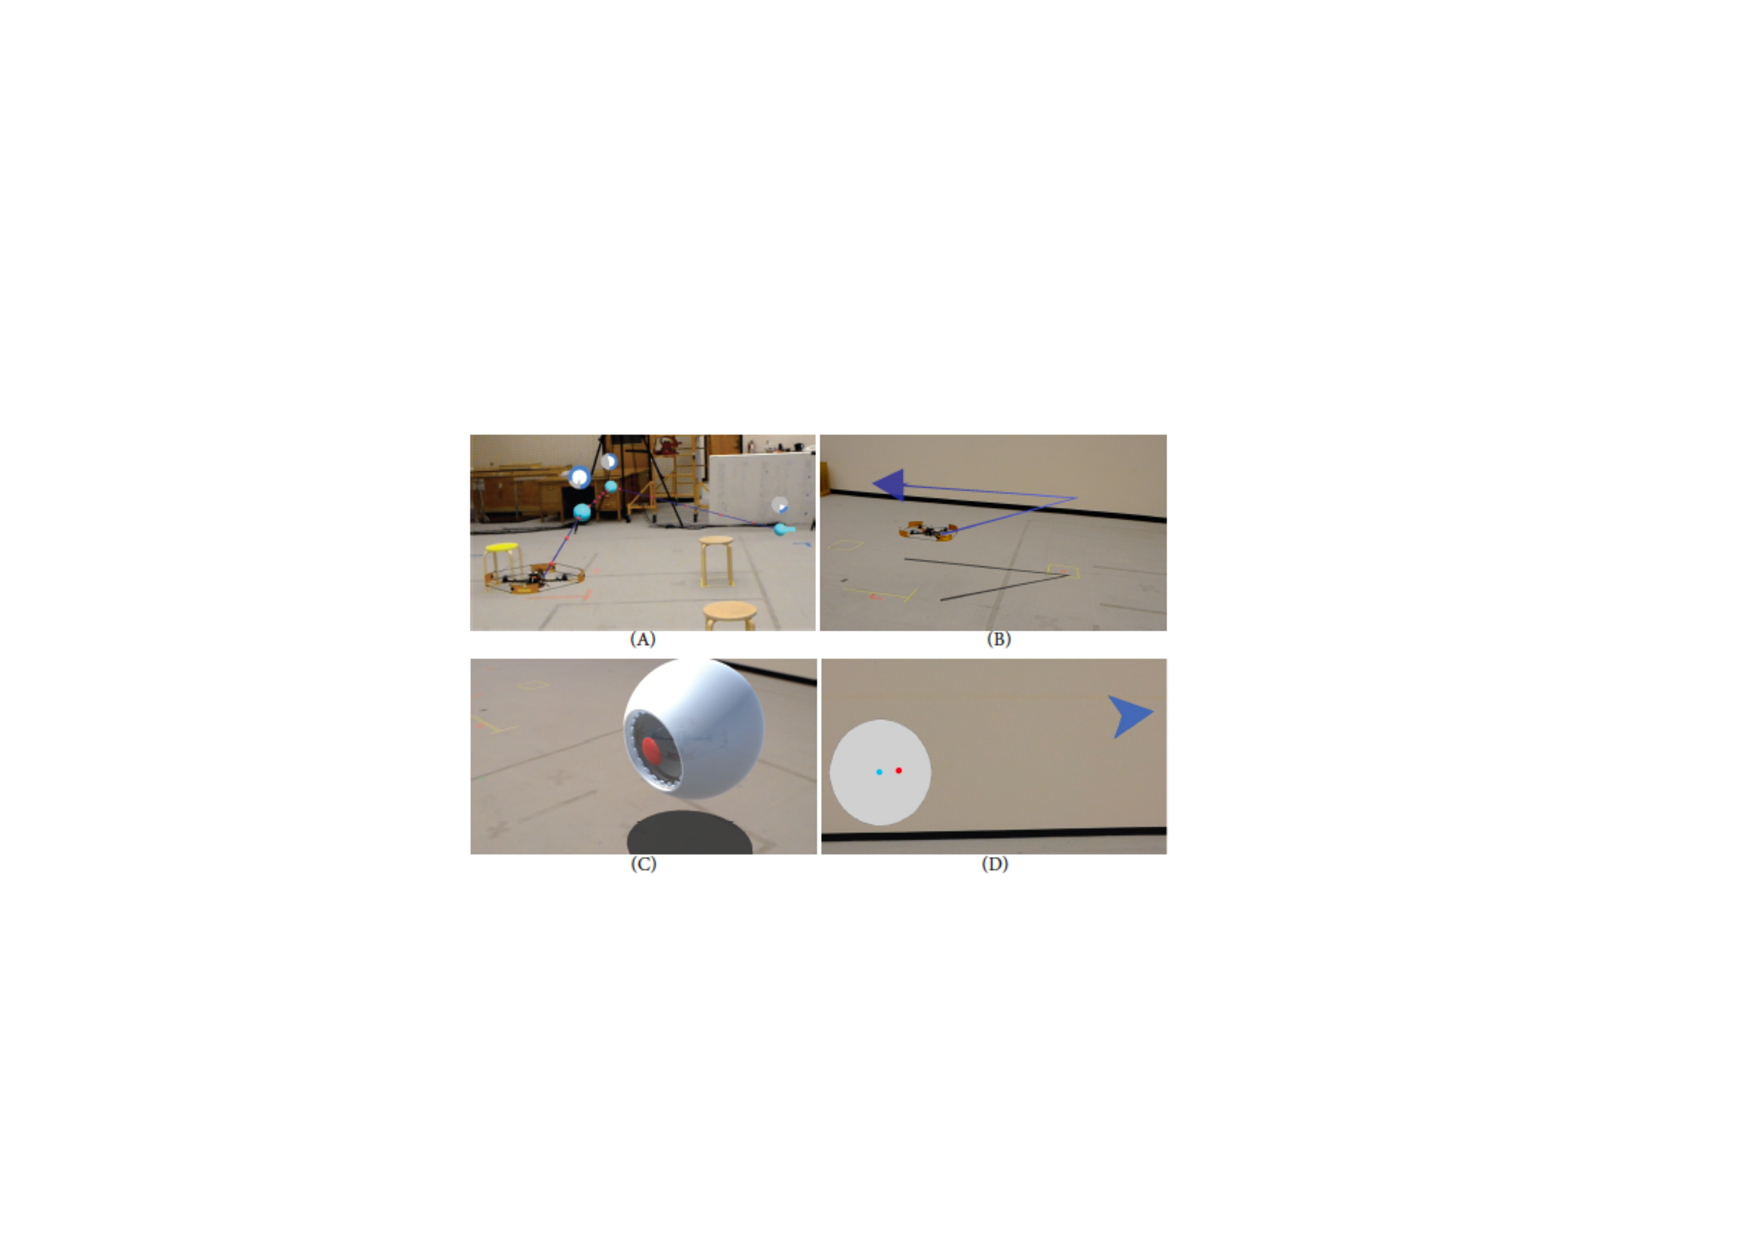
\includegraphics[width=\linewidth]{img/overview_hi.pdf}
  \caption{ARインタフェースの例}
  \label{fig:arinterface}
  \vspace{-3mm}
\end{figure}

\begin{figure*}[!tb]
  \centering
  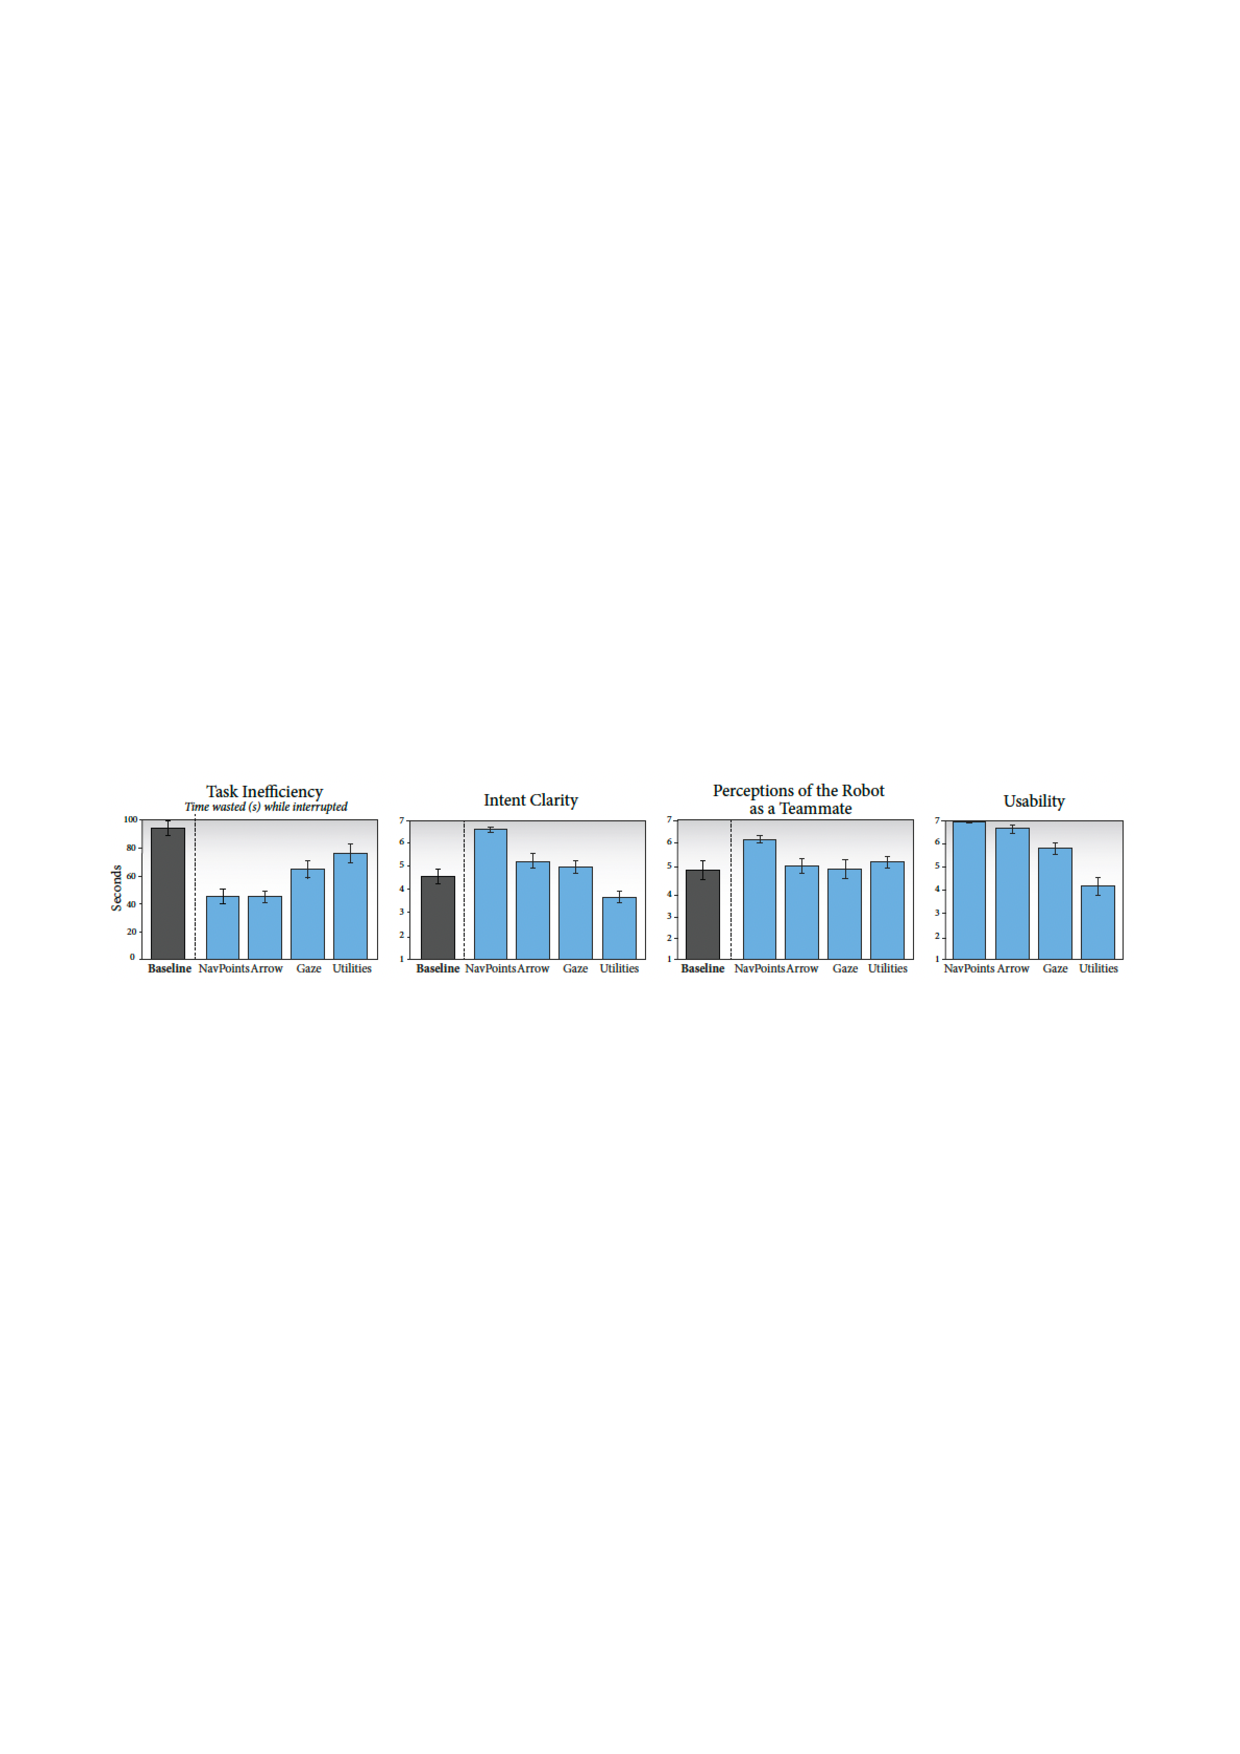
\includegraphics[width=\linewidth]{img/result.pdf}
  \caption{実験結果}
  \label{fig:result}
  \vspace{-3mm}
\end{figure*}

%---------------------------------------------------------------------

\subsection{Utilities}
% 最後のデザインは,ユーザインタフェースを拡張して,自分を中心とした文脈情報を提供する方法の可能性を示しています.
% このデザインは,パイロット・インターフェース[24],ドローン制御インターフェース[28],ビデオゲーム・インターフェース[32,34],軍事用途[15]などでよく用いられる,
% ミニマップ,レーダー,オフスクリーン・インジケータなどの周辺ユーティリティにヒントを得ています.
Utilitiesデザインでは,ARHMDのディスプレイ左下にレーダを表示する.
このレーダ上ではユーザは中心に青い点で,ドローンは赤い点で表示され,赤い点の大きさは,ドローンの現在の高度に正比例している.
% レーダーの検出半径Xは,インターフェース設計者がカスタマイズすることも,ユーザーが調整することもできる.
また,ドローンがユーザの視野内に入っている間は,ターゲティングボックスで強調表示され,
視野外に出た場合は,
% 画面外のインジケータが方向矢印の形で表示される.
ARHMDディスプレイの端に画面外のドローンの位置を示す矢印が表示される.
本デザインはユーザは相対的なドローンの位置を素早く確認することができる.

%---------------------------------------------------------------------

\section{評価}\label{experiment}
\subsection{概要}
本研究では,ワークスペースでのドローンとのインタラクションにARデザインがどのような影響を与えるかを評価した.
実験では,提案していたARを用いてデザインフレームワーク4つとARを用いないベースライン条件の計5つの手法を用いて行った.
ベースライン条件では,他の条件と同じ環境を維持するため,参加者はARHMDを装着しているが,AR表示はされていない.
また,ドローンには明確な「正面」があり,それは常に進行方向を示している.
% この基本動作はすべての条件で共通している.


\subsection{実験環境}
実験は,20フィート×35フィート×20フィートの大きさの環境で行った.
環境内には6台の作業場が3台ずつ2列に配置される.
各ワークステーションの周囲には,最低5フィートの自由空間があり,カラービーズの容器が置かれている.

\subsection{タスク}
各ビーズ容器には,緑,黒,黄,白,青,赤のいずれか1色のビーズしか入っておらず,
参加者は,ドローンに見つかることなく,これらの容器からビーズを集めてつなぎ合わせ,
できるだけ多くのビーズの紐を作る課題を与えられた.
それぞれの紐には,
例えば,青のビーズを10個,赤のビーズを5個,緑のビーズを10個,というように
目標とする色と使用するビーズの量が指示された.
これらの指示に加えて,参加者には3つのルールが指示された.
\begin{enumerate} % 箇条書きは \begin{itemize}
  \item ビーズは一度に1つのみ拾え,ワークステーションにいる間はビーズを紐に置くことしかできない
  \item どのような順番でも色を集めることができるが,一度色を選べば
        紐の指示通りにその色のビーズをすべて繋ぎ終えるまでその色のステーションに留まらなければならない
  \item 参加者は作業中のワークステーションにロボットが飛んできた場合,ワークステーションから最低2メートル離れ,
        ロボットが去るまで待たなければならない
\end{enumerate}


\subsection{評価}
コロラド大学ボルダー校から60名の参加者(男性40名,女性20名,条件は均等)を募集し,
平均年齢は20.7歳(SD = 4.8)で,18~45歳の範囲であった.
実験を通して,タスクのパフォーマンスと効率の客観的評価,およびコミュニケーションの明瞭さとドローンの使いやすさの主観的評価を行った.
図\ref{fig:result}は,これらの結果をまとめたものである.
\subsection{評価結果}
客観的結果では,割り込みによる総損失時間を評価した.
主観的結果では,コミュニケーションの明確さ,ドローンを共同作業のパートナーとして見れるか
AR表示が参加者のドローン動作意図の理解にどのように影響するかの3点を評価した.
図\ref{fig:result}より,「NavPoints」,「Arrow」,「Gaze」は,非効率性を低減することでタスクパフォーマンスを向上させた.
参加者は,ドローンの意図をより的確に予測し,それに応じて自分の行動を計画することで,中断や非生産的な時間を減らすことができた.


%---------------------------------------------------------------------
\section{まとめ}
効果的な共同作業には自分たちの意図を迅速かつ正確に伝える必要がある.
本論文ではARを利用し,特に空中ドローンにおいて,ドローンの動作意図を同じ場所にいるユーザーに伝える4つの手法について,比較・評価を行なった.
その結果,「NavPoints」,「Arrow」,「Gaze」はドローンの使いやすさや受け入れ意欲向上につながることが実証された.
また,「NavPoints」はすべての尺度で一貫して高い評価を得ており,ドローンの飛行経路および到着と出発を明示的に表現することが,
ユーザのタスクパフォーマンスを最も向上させることがわかった.
%---------------------------------------------------------------------


% \subsection{表}
% 表は\tabref{tab:data_type}のように引用することができ,表を作成する場合は罫線を少なくすることと,横線のみの使用を心がけることが推奨される.

% \begin{table}[!bt]
%   \caption{代表的なデータの型}
%   \label{tab:data_type}
%   \centering
%   \begin{tabular}{lcr}
%     \hline
%     データの型         & 宣言   & ビット幅 \\
%     \hline \hline
%     短整数型           & short  & 16       \\
%     整数型             & int    & 32       \\
%     単精度浮動小数点型 & float  & 32       \\
%     倍精度浮動小数店型 & double & 64       \\
%     \hline
%   \end{tabular}
% \end{table}

%---------------------------------------------------------------------
% \section{研究者にとっての論文十箇条}
% 論文を書くことは大切だ必要だ,と周囲から言われる.それは自分でも分かっているつもりだけれど,その理由をはっきりと伝えてもらえる機会は少ない.研究者にとっての論文十箇条\cite{whats_paper}は,とてもシンプルでわかりやすく,非常に心にきた.一度目を通してみるべきであろう.

% \begin{enumerate} % 箇条書きは \begin{itemize}
% \item 書かれた論文は書いた人の研究者としての人格を表す
% \item データのみ出して論文を書かない者は,テクニシャンである
% \item データも出さず,論文(原著論文)を書かない者は,評論家である
% \item 研究者は論文を書くことによって成長する.また,成長の糧にしなければならない
% \item 論文は研究者の飯のタネである
% \item 論文は後世の研究に影響を与えなければならない
% \item 研究者は書いた論文に責任を問われる
% \item 忙しくて論文が書けないというのは,言い訳にはならず,能力がないといっているのと同じである
% \item 博士論文以上の論文を書けない者は,その博士論文は指導教官のものといわれても仕方がない
% \item 研究において最も重要なのはアイデアであり,それが試されるのが論文である
% \end{enumerate}

%---------------------------------------------------------------------
% Bibliography
\footnotesize{
  \begin{thebibliography}{99}
    \bibitem{main} M. Walker, H. Hedayati, J. Lee and D. Szafir, Communicating Robot Motion Intent with Augmented
    Reality, HRI ’18: Proceedings of the 2018 ACM/IEEE International Conference on Human-Robot
    Interaction, pp.316-324, 2018, doi:10.1145/3171221.3171253.
  \end{thebibliography}
}

%---------------------------------------------------------------------
\end{document}
%---------------------------------------------------------------------
